\documentclass[tikz,border=5pt]{standalone}
\usepackage{fontspec}
\setmainfont{Times New Roman}
\usepackage{unicode-math}
\setmathfont{Cambria Math}
\usetikzlibrary{shapes.geometric,shapes.misc,positioning,fit,backgrounds,arrows.meta,calc}

\begin{document}
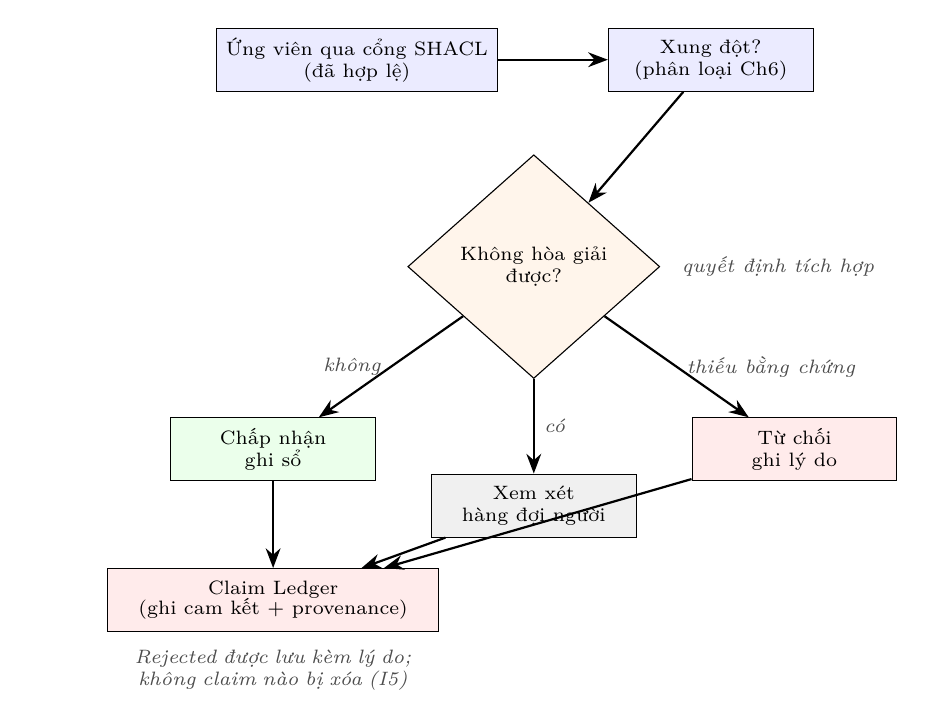
\begin{tikzpicture}[
    node distance=1.1cm and 1.4cm,
    box/.style={rectangle, draw, minimum width=2.6cm, minimum height=0.8cm, align=center, font=\scriptsize},
    label/.style={font=\scriptsize\itshape, text=gray!60!black},
    arrow/.style={-{Stealth[length=2.5mm]}, thick},
]

% ====== Inputs ======
\node[box, fill=blue!8] (gate) at (0, 3.2) {Ứng viên qua cổng SHACL\\
\scriptsize(đã hợp lệ)};
\node[box, fill=blue!8, right=of gate] (conflict) {Xung đột?\\
\scriptsize(phân loại Ch6)};

\draw[arrow] (gate) -- (conflict);

% ====== Decision diamond ======
\node[diamond, draw, fill=orange!8, minimum width=3.2cm, minimum height=1.6cm, align=center, font=\scriptsize, below=1.2cm of $(gate)!0.5!(conflict)$] (dec) {Không hòa giải\\được?};

\draw[arrow] (conflict) -- (dec);

\node[label, right=0.15cm of dec, align=left] (q) {quyết định tích hợp};

% ====== Three branches ======
\node[box, fill=green!8, below left=1.2cm and 1.2cm of dec] (accept) {Chấp nhận\\
\scriptsize ghi sổ};
\node[box, fill=gray!12, below=1.2cm of dec] (defer) {Xem xét\\
\scriptsize hàng đợi người};
\node[box, fill=red!8, below right=1.2cm and 1.2cm of dec] (reject) {Từ chối\\
\scriptsize ghi lý do};

\draw[arrow] (dec) -- node[label, left, pos=0.5] {không} (accept);
\draw[arrow] (dec) -- node[label, right, pos=0.5] {có} (defer);
\draw[arrow] (dec) -- node[label, right, pos=0.5] {thiếu bằng chứng} (reject);

% ====== Ledger ======
\node[box, fill=red!8, minimum width=4.2cm, below=1.1cm of accept] (ledger) {Claim Ledger\\[-1pt]\scriptsize(ghi cam kết + provenance)};

\draw[arrow] (accept) -- (ledger);
\draw[arrow] (defer) -- (ledger);
\draw[arrow] (reject) -- (ledger);

\node[label, below=0.1cm of ledger, align=center, text width=6cm]
{Rejected được lưu kèm lý do; không claim nào bị xóa (I5)};

\end{tikzpicture}
\end{document}